\documentclass{article}
\usepackage{amsmath, amssymb, kotex, hyperref, graphicx, mdframed, setspace}
\usepackage[a4paper, margin = 40pt]{geometry}
\setstretch{1.5}
\begin{document}
\title{시계열 회귀분석(Time Series Regression - 2)}
\author{강의 : 김성범 교수님\\ 정리 :  김선중}
\date{\today}
\maketitle

이것은 \href{https://youtu.be/pxG4ZlHJ570}{Time Series Regression - Part 2} 강의에 대한 노트이다.
\tableofcontents

\newpage

%%
\section{오차와 잔차(errors and residuals)}
%%%
\subsection{추정에서의 오차와 잔차}
임의추출을 통해 모평균을 추정하는 문제를 생각할 때, 어떤 표본 \(X_i\)에 대하여, \(X_i\)와 모평균 \(\mu\) 사이의 차를 오차(error, \(e_i\))라고 한다.
\[e_i = X_i-\mu.\]
하지만, 실제 상황에서는 모평균을 안다는 것은 불가능하다.
그래서 모평균 대신 표본평균인 \(\overline X = \frac{X_1+\cdots+X_n}n\)을 사용해 그 차이를 계산할 수 있는데, 그 값이 잔차(residual, \(\epsilon_i\))이다.
\[\epsilon_i = X_i-\overline X.\]
%%%
\subsection{회귀에서의 오차와 잔차}
회귀(regression)란, 독립변수 \(x\)와 종속변수 \(y\)에 대하여 관측값(observed value)들이 주어져 있을 때, 두 변수 사이의 관계를 찾는 것이다.
조금 더 정확하게는, \(y\)를 \(x\)에 대한 함수 \(y=f(x)\)로서 표현하는 것이다.
관측값은 다음과 같이 주어질 것이다.
\[\text{관측값} = \{(x_i,y_i):i=1,2,\cdots,n\}.\]
일부 \(x\)값들에 대해서만 \(y\)값들이 주어져있으므로 함수 \(f\)를 완벽하게 안다는 것은 불가능하다.
대신, 관측값들을 토대로 하여 만든 최적의 함수 \(\hat f\)를 생각하게 된다.
이때, 관측값 \(y_i\)에 대한 오차(error, \(e_i\))와 잔차(residual, \(\epsilon_i\))는 다음과 같다.
\begin{align}
e_i&=y_i-f(x_i)\label{error}\\
\epsilon_i&=y_i-\hat f(x_i)\label{residual}
\end{align}
예측값인 \(\hat f(x_i)\)는 \(\hat y_i\)라고 쓰기도 하므로, 잔차를 다음과 같이 쓰기도 한다.
\[\epsilon_i=y_i-\hat y_i.\]

최적의 함수 \(\hat f\)를 찾아가는 과정은 다음과 같다.
먼저, 여러 개의 매개변수 \(\beta_0\), \(\beta_1\), \(\beta_2\), \(\cdots\), \(\beta_k\)를 통해 함수 \(f_\beta\)를 정의한다.
\footnote{여기서 \(\beta\)는 매개변수 \(\beta_i\)들의 집합이라는 의미에서 썼다.
머신러닝에서 \(\Theta\)를 매개변수 \(w_{ij}\), \(b_i\)들의 집합으로 자주 표현하듯이.
그러니까, 굳이 식으로 써보자면 \(\beta=\{\beta_0,\beta_1,\cdots,\beta_k\}\)이 된다.}
즉, 함수 \(f_\beta\)는 parametric function/model 이다. (resp. nonparametric function/model).
그리고, 그러한 \(f_\beta\)들 중에서 관측값들을 가장 잘 반영하는 함수 \(\hat f\)를 찾는다.
다시 말해, 전체적으로 \(y_i\)와 \(f(x_i)\)가 가장 비슷해지는 \(\beta_0,\beta_1,\cdots,\beta_k\)을 찾는데, 이때에 `비슷함'의 기준은 MSE 등을 통해 정할 수 있다.
가장 비슷해지는 때의 \(\beta_0,\beta_1,\cdots,\beta_k\)는, hat을 붙여서 \(\hat\beta_0,\hat\beta_1,\cdots,\hat\beta_k\)로 표현한다.
그리고 이 매개변수(parameters)들을 가지고 최적의 함수 \(\hat f =  f_{\hat\beta}\)를 정의한다.

%%
\section{여러가지 회귀모델}
(앞서 말했듯이) 회귀란, 관측값들 \(\{(x_i,y_i):i=1,2,\cdots,n\}\)로부터 \(x\)와 \(y\) 사이의 관계식을 \(y=\hat f(x)\)으로 추정해나가는 것이다.
시계열 데이터를 다루는 만큼 index를 \(i\) 대신 \(t\)라고 쓰고, \(\hat f(x)\)를 추세(trend)를 뜻하는 $TR$이라는 기호로 고쳐 쓰면 식 \eqref{error}는 다음 식이 된다.
\[y_t=TR_t+\epsilon_t.\]
이 표기방식은 강의에서 나온 방식인데, 그것보다는, 위의 설명과의 통일성을 위해 아래와 같이 쓰는 것도 괜찮을 것 같다.
\[y_t=\hat f(x_t)+\epsilon_t.\]
%\begin{quotation}
%Time series \(y_t\) can be represented by an average level that changes over time according to the equation \(TR_t\) and by the error term.
%\end{quotation}

%%%
\subsection{상수회귀(no trend)}
상수함수 \(f_\beta(x)=\beta_0\)를 생각하자.
아까 말했듯이, 이것은 parametric function이다.
즉 매개변수(parameter) \(\beta_0\)에 의해 결정되는 함수이다.
이러한 \(f_\beta\) 중에서 최적의 \(\hat f\)를 구한다는 것은, 다음과 같은 MSE 값이 최소가 되는 때를 찾는 것이다.
\begin{align*}
MSE(\beta_0)
& = \frac1n\sum_{t=1}^n(y_t-f_\beta(x_t))^2\\
& = \frac1n\sum_{t=1}^n(y_t-\beta_0)^2
\end{align*}
이때, MSE는 \(\beta_0\)의 값에만 의존한다.
조금 더 정확하게는, MSE는 \(\beta_0\)에 대한 이차함수이다.
이 이차함수의 최솟값은 중학교 3학년 과정의 방식으로 풀어도 되기는 하지만, 미분해서 0이 되는 때를 구해도 상관없다;
\begin{gather*}
\frac{d}{d\beta_0}MSE(\beta_0)=0\\
-\frac2n\sum_{t=1}^n(y_t-\beta_0)=0\\
\sum_{t=1}^ny_t-n\beta_0=0\\
\beta_0=\frac1n\sum_{t=1}^ny_t.
\end{gather*}
%\(y_t\)들의 평균을 간단히 \(\bar y\)라고 쓰면,
즉, \(\hat\beta_0=\frac1n\sum_{t=1}^ny_t\)이고, \(\hat f(x)=\frac1n\sum_{t=1}^ny_t\)이다.
강의에서는 상수회귀에 대한 예를 들고 있고, 더 나아가 point estimate와 confidence interval 같은 것도 이야기하고 있다.

%%%
\subsection{선형회귀(linear trend, linear regression)}
일차함수 \(f_\beta(x)=\beta_0+\beta_1x\)를 생각하자.\footnotemark
\footnotetext{정확하게는 일차함수(linear function)라는 표현보다는 `affine 함수(affine function)'라고 써야 더 맞을 것 같다.}
이것도 parametric function이다.
즉, \(\beta_0\)와 \(\beta_1\)에 의해 결정되는 함수이다.
이번에도 \(\hat f\)를 구하기 위해 MSE가 최솟값이 되는 때를 찾는다.
다만, 이번에는 MSE가 두 매개변수 \(\beta_0\), \(\beta_1\)의 함수이다.
\[MSE(\beta_0,\beta_1)=\frac1n\sum_{t=1}^n(y_t-\beta_0-\beta_1x)^2\]
이것은 다변수함수라는 점에서는 아까보다 훨씬 복잡한 함수이지만, 이차함수라는 점에서는 간단하다.
아래로 볼록한 포물면을 그래프로 가지고, 단 하나의 극솟값을 가지므로 이 함수가 극솟값(local minimum)을 가지게 되는 \((\beta_0, \beta_1)\)만 찾으면 그때가 최소점(global minimum)이 된다.
그리고 그건 MSE를 두 매개변수 \(\beta_0\), \(\beta_1\)로 각각 편미분하여 0이 되는 때이다.
먼저 \(\frac{\partial}{\partial\beta_0}MSE(\beta_0,\beta_1)=0\)를 간단히하면
\begin{gather*}
\frac{\partial}{\partial\beta_0}MSE(\beta_0,\beta_1)=0\\
-\frac2\sum_{t=1}^n(y_t-\beta_0-\beta_1x_t)=0\\
\sum_{t=1}^ny_t-n\beta_0-\beta_1\sum_{i=1}^nx_t=0
\end{gather*}
이고, \(\frac{\partial}{\partial\beta_1}MSE(\beta_0,\beta_1)=0\)를 간단히하면
\begin{gather*}
\frac{\partial}{\partial\beta_1}MSE(\beta_0,\beta_1)=0\\
-\frac2n\sum_{t=1}^nx_t(y_t-\beta_0-\beta_1x_t)=0\\
\sum_{t=1}^nx_ty_t-\beta_0\sum_{t=1}^nx_t-\beta_1\sum_{t=1}^n{x_t}^2=0
\end{gather*}
따라서
\[
\begin{bmatrix}
n&\sum x_t\\
\sum x_t&\sum{x_t}^2
\end{bmatrix}
\begin{bmatrix}
\beta_0\\\beta_1
\end{bmatrix}
=
\begin{bmatrix}
\sum y_t\\\sum x_ty_t
\end{bmatrix}
\]
를 풀면 \(\hat\beta_0\)와 \(\hat\beta_1\)을 구할 수 있다.
%그리고 좌변의 정사각행렬은 항상 역행렬이 존재하므로, 위의 연립방정식은 항상 풀린다.
이렇게 하면, 최적의 함수 \(\hat f(x)=\hat\beta_0+\hat\beta_1x\)를 얻어낼 수 있다.

%%%
\subsection{이차회귀(quadratic trend, quadratic regression)}
이차함수 \(f_\beta(x)=\beta_0+\beta_1x+\beta_2x^2\)를 생각하자.
위와 마찬가지로
\[MSE(\beta_0,\beta_1,\beta_2)=\frac1n\sum_{t=1}^n(y_t-\beta_0-\beta_1{x_t}-\beta_2{x_t}^2)^2\]
이다.
이것은 \(\beta_0\), \(\beta_1\), \(\beta_2\)에 대한 함수이다.
각각의 매개변수 \(\beta_0\), \(\beta_1\), \(\beta_2\)에 대한 편미분값을 0으로 둠으로써 연립방정식을 얻고,
\begin{gather*}
\sum_{t=1}^ny_t-n\beta_0-\beta_1\sum_{t=1}^nx_t+\beta_2\sum_{t=1}^n{x_t}^2=0\\
\sum_{t=1}^nx_ty_t-\beta_0\sum_{t=1}^nx_t-\beta_1\sum_{t=1}^n{x_t}^2+\beta_2\sum_{t=1}^n{x_t}^3=0\\
\sum_{t=1}^n{x_t}^2y_t-\beta_0\sum_{t=1}^n{x_t}^2-\beta_1\sum_{t=1}^n{x_t}^3+\beta_2\sum_{t=1}^n{x_t}^4=0\\
\begin{bmatrix}
n&\sum x_t&\sum{x_t}^2\\
\sum x_t&\sum{x_t}^2&\sum{x_t}^3\\
\sum{x_t}^2&\sum{x_t}^3&\sum{x_t}^4\\
\end{bmatrix}
\begin{bmatrix}
\beta_0\\\beta_1\\\beta_2
\end{bmatrix}
=
\begin{bmatrix}
\sum y_t\\\sum x_ty_t\\\sum{x_t}^2y_t
\end{bmatrix}
\end{gather*}
이 식을 풀면, MSE가 최소가 되는 \(\beta_0\), \(\beta_1\), \(\beta_2\)를 계산할 수 있다.

%%%
\subsection{다항회귀(polynomial trend, polynomial regression)}
마찬가지로, 다항함수 \(f_\beta(x)=\beta_0+\beta_1x+\beta_2x^2+\cdots+\beta_kx^k\)를 parametric model로 잡으면
\[MSE(\beta_0,\beta_1,\beta_2,\cdots,\beta_k)=\frac1n\sum_{t=1}^n(y_t-\beta_0-\beta_1x-\beta_2x^2-\cdots-\beta_kx^k)^2\]
이고, 똑같은 작업을 통해 \(\hat f(x)=\hat \beta_0+\hat \beta_1x+\hat \beta_2x^2+\cdots+\hat \beta_kx^k\)를 계산할 수 있다.

\textbf{2.1 \(\sim\) 2.4}에서와 같이, \(\hat f\)를 계산하는 방식을 최소제곱법(최소자승법, least square method, least square estimation, the method of least square)이라고 한다.
또한, 지금까지 한 것은 한 변수에 대한 회귀(univariate regression)였다.
일반적으로는 다변수에 대해서도 회귀(multivariate regression)를 진행할 수 있다.
변수들을 \(x_1\), \(x_2\), \(\cdots\), \(x_k\)이라고 하면 parametric model \(f_\beta(x_1,x_2,\cdots,x_k)\)을 생각할 수 있다.
가장 간단한 경우는 다변수 선형회귀(multivariate linear regression)일 것이고, 그것은 parametric model을
\[f_\beta(x_1,x_2,\cdots,x_k)=\beta_0+\beta_1x_1+\cdots+\beta_kx_k\]
로 두는 것이다.
이 때에도 마찬가지로 최소제곱법을 사용해서 \(\hat f\)를 계산할 수 있다.

%%
\section{자기상관성(autocorrelation)}
회귀문제에서 각각의 오차(\(e_t\))들에 대하여 전제되어야 하는 몇가지 가정들이 있었다.\footnote{왜 이런 가정이 필요한지는 아직 이해하지 못했다.
하지만 `아래의 두 가정을 따르도록 하는 \(f_\beta\)를 고려하겠다.' 정도로 생각해도 될 것 같다.}
\begin{itemize}
\item
\(e_t\sim N(0,\sigma^2)\) : 오차는 평균이 0인 정규분포를 따른다.
\item
\(t\neq s\)이면 \(e_t\)와 \(e_s\)는 서로 독립이다.
\end{itemize}
그런데 우리가 다룰 시계열데이터의 경우, 이러한 전제가 성립되지 않을 가능성이 있다.
즉, 각각의 \(e_t\)에 대하여, \(e_t\)들이 서로 독립이 아닌 종속의 관계를 따를 수 있고, 그렇게 된다면, 최소제곱법과 같은 풀이법을 사용할 수 없을 지도 모른다.
그리고, 실제로는 오차(\(e_t\))를 계산할 수 없으므로 대신 잔차(\(\epsilon_t\))의 독립성/종속성을 계산한다.
여기에서는 공분산과 피어슨 상관계수에 대해 복습하고, 자기상관성에 대해 알아본다.

%%%
\subsection{공분산(covariance)}
두 확률변수 \(X\), \(Y\)에 대하여, \(X\)와 \(Y\)의 공분산(correlation) \(\text{Cov}(X,Y)\)는  다음과 같이 정의된다.
\begin{equation}
\text{Cov}(X,Y)=\mathbb E[(X-\mathbb E[X])(Y-\mathbb E[Y])]
\end{equation}
\(\mathbb E\)는 linear operator이므로
\begin{align*}
\text{Cov}(X,Y)
&=\mathbb E[(X-\mathbb E[X])(Y-\mathbb E[Y])]\\
&=\mathbb E[(X-\mu)(Y-\nu)]\\
&=\mathbb E[XY]-\mu\mathbb E[Y]-\nu\mathbb E[X]+\mathbb E[\mu\nu]\\
&=\mathbb E[XY]-\mu\nu-\mu\nu+\mu\nu\\
&=\mathbb E[XY]-\mathbb E[X]\mathbb E[Y]
\end{align*}
라고 쓸 수도 있다.
만약 \(X\), \(Y\)가 독립이면, \(\mathbb E(XY)=\mathbb E(X)\mathbb E(Y)\)이므로, \(\text{Cov}(X,Y)=0\)이 되고 그 역도 성립한다.

관측치 \(\{(x_t, y_t):t=1,2,\cdots,n\}\)에 대한 공분산은
\[\text{Cov}(X,Y)=\frac1{n-1}\sum_{t=1}^n(x_t-\mu)(y_i-\nu)\]
으로 계산하면 되는 것 같다.
당연한 말이지만 \(Y=X\)이면 공분산은 분산이 된다 ; \(\text{Cov}(X,X)=V(X)\).
공분산에 대한 일반적인 설명과 여러가지 예제들은 \href{https://youtu.be/qtaqvPAeEJY}{StatQuest:Covariance, Clearly Explained}에 가장 친절하게 설명되어 있는 것 같다.

%%%
\subsection{피어슨 상관계수(correlation)}
두 확률변수 \(X\), \(Y\)에 대하여 \(X\), \(Y\)의 피어슨 상관계수는 
\begin{equation}\label{pearson1}
\text{Cor}(X,Y)=\frac{\text{Cov}(X,Y)}{\sigma[X]\sigma[Y]}=\frac{\mathbb E[(X-\mathbb E[X])(Y-\mathbb E[Y])]}{\sigma[X]\sigma[Y]}
\end{equation}
이다.
\(\text{Cor}(X,Y)\)는 \(-1\)과 \(1\) 사이의 값을 가지는데 그것은 Cauchy-Schwarz 부등식 \(|v|\cdot|w|\le|v\cdot w|\)으로 쉽게 증명된다.
\footnote{\(X\), \(Y\)가 이산확률변수인 경우만 고려했는데, 연속확률변수인 경우에도 비슷하게 증명될 수 있을 것이다.}
\begin{align*}
\bigg|\mathbb E\left[\left(X-\mathbb E[X]\right)\left(Y-\mathbb E[Y]\right)\right]\bigg|
&=\frac1{n-1}\left|\sum_{t=1}^n(x_i-\mu)(y_i-\nu)\right|\\
&=\frac1{n-1}\left|(x_1-\mu,\cdots,x_n-\mu)\cdot(y_1-\nu,\cdots,y_n-\nu)\right|\\
&\le\frac1{n-1}\left|(x_1-\mu,\cdots,x_n-\mu)\right|\cdot\left|(y_1-\nu,\cdots,y_n-\nu)\right|\\
&=\sigma(X)\sigma(Y)
\end{align*}
관측치 \(\{(x_i, y_i):i=1,2,\cdots,n\}\)에 대한 피어슨 상관계수는
\begin{equation}\label{pearson2}
\text{Cor}(X,Y)
=\frac{\frac1{n-1}\sum_{t=1}^n(x_t-\mu)(y_i-\nu)}{\sqrt{\frac1{n-1}\sum_{t=1}^n(x_t-\mu)^2}\sqrt{\frac1{n-1}\sum_{t=1}^n(x_t-\mu)^2}}
=\frac{\sum_{t=1}^n(x_t-\mu)(y_i-\nu)}{\sqrt{\sum_{t=1}^n(x_t-\mu)^2}\sqrt{\sum_{t=1}^n(x_t-\mu)^2}}
\end{equation}
으로 계산하면 되는 것 같다.
피어슨 상관계수에 대한 일반적인 설명과 여러가지 예제들은 \href{https://youtu.be/xZ_z8KWkhXE}{StatQuest:Pearson's Correlation, Clearly Explained}에 가장 친절하게 설명되어 있는 것 같다.
관측치의 \(n\)개 점들이 모두 한 직선 위에 있으면, 피어슨 상관계수는 (기울기가 양수일 경우) 1이거나 (기울기가 음수일 경우) $-1$이다.

%%%
\subsection{자기상관성(autocorrelation)}
시계열 데이터 \(X=\{x_t:t=1,2,\cdots, n\}\)는 길이가 \(n\)인 수열이라고 생각할 수 있다.
이 시계열데이터를 timestep 1만큼 shift 시켜서 \(X'=\{x_t:t=2,3,\cdots, n+1\}\)를 만들자.
\(X\)의 첫항과 \(X'\)의 마지막 항을 제외하고, \(X\)와 \(X'\)의 항들을 대응시키면
\[\{(x_t,x_{t+1}):t=1,2,\cdots,n-1\}\]
는 하나의 `관측치'가 된다.
이것에 대한 피어슨 상관계수를 자기상관성이라고 한다.
\footnote{그런데 \(X\)에 대한 자기상관성이 왜 나오는지 잘 모르겠(었)다.
\textbf{3.1.}의 앞에서 설명한 것은 오차 \(e_t\)들 사이의 독립/종속성이었지 \(X\)와 \(X'\)의 독립/종속성은 아니었다.
다시 생각해보면, 강의에서는 `일반적인' 자기상관성의 정의에 대해 설명하고 있지만, 오차 \(e_t\)에 대한 자기상관성은, 여기서 설명하는 자기상관성의 정의에 적용할 수 있다.
강의의 27분 15초 부터 이에 대한 설명이 있다.

우리가 관심있는 것은, error term에 대한 자기상관성이다.
만약, error term의 자기상관성이 0이어서, 각 timestep마다의 error term \(e_t\)가 서로 독립적이면, 기존의 방법인 `다변수회귀'의 방법을 그대로 써도 되고, 만약 자기상관성이 0이 아니어서 \(e_t\)가 서로 종속적이라면, 다변수회귀가 아닌 다른 방법을 강구해야 한다.
하지만, 실제 상황에서 오차 \(e_t\)는 계산할 수 없으므로, 대신 잔차 \(\epsilon_t\)를 고려한다. (the residuals are point estimates of the error terms.)
그리고 잔차의 자기상관성을 계산함으로써, 오차가 자기상관성을 가지는 지의 여부를 판단하게 된다. (a residual plot against time can be used to detect the violence of the independence assumption.)}
%강의에서는, 관측치에서의 첫번째 성분을 \(X\), 뒤의 성분을 \(X'\)이라고 썼다.
%그러니까, 
%\begin{align*}
%X&=\{x_t:t=1,2,\cdots,n\}\\
%X'&=\{x_{t+1}:t=1,2,\cdots,n\}
%\end{align*}
%이라고 생각하자.
그러면 자기상관성(autocorrelation of order 1) \(\rho_1(X)\)은\footnotemark
\begin{equation}\label{autocorrelation}
\rho_1(X)=\text{Cor}(X,X')
\end{equation}
인 것이다.
\footnotetext{autocorrelation을 표현하는 표기 방식은 책마다 문헌마다 다 다른 것 같다.
여기에서는 영상의 29분 45초경에 나오기도 하고, 위키피디아에 쓰여져있기도 한 \(\rho\)(rho)를 사용했다.
아래첨자로 1을 넣은 것은 order=1이라는 의미이고 여기에서의 order는 lag를 의미한다.
lag=2이면 second order, lag=3이면 third order와 같이 쓴다고 강의에 설명되어 있다.}

이게 뭔지 잘 와닿지가 않아서, 몇 개의 예를 만들어보았다.
\(n=6\)이고 \(X\)가 선형적으로 증가하는 경우를 생각해보았다.
\begin{center}
\begin{tabular}{c|ccccccc}
$X$ &1&2&3&4&5&6&\\\hline
$X'$& &1&2&3&4&5&6
\end{tabular}
\end{center}
자기상관성을 계산하기 위해서는, 관측치
\[\{(2,1),(3,2),(4,3),(5,4),(6,5)\}\]
에 대한 피어슨 상관계수를 계산하면 된다.
이 다섯 개의 점들은 한 직선 위에 있으므로 \(\text{Cor}(X,X')=1\)이 되어야 한다.
실제 계산을 해보아도 (식 \eqref{pearson2})
\begin{align*}
\text{Cor}(X,X')
&=\frac{(2-4)(1-3)+(3-4)(2-3)+(4-4)(3-3)+(5-4)(4-3)+(6-4)(5-3)}{\sqrt{(2-4)^2+(3-4)^2+(4-4)^2+(5-4)^2+(6-4)^2}\sqrt{(1-3)^2+(2-3)^2+(3-3)^2+(4-3)^2+(5-3)^2}}\\
&=\frac{10}{\sqrt{10}\sqrt{10}}=1.
\end{align*}
이 된다.
다시 말해서, 선형적인 시계열과 그것을 shift시킨 것은 1의 상관성을 가진다.

이번에는 $n=6$이고 $X$가 quadratic하게 증가하는 경우를 생각해보았다.
\begin{center}
\begin{tabular}{c|ccccccc}
$X$ &0&1&4&9&16&25&\\\hline
$X'$& &0&1&4&9&16&25
\end{tabular}
\end{center}
자기상관성을 계산하기 위해서는, 관측치
\[\{(1,0),(4,1),(9,4),(16,9),(25,16)\}\]
에 대한 피어슨 상관계수를 계산하면 된다.
이 다섯 개의 점들은 양의 상관관계가 있기는 해도 한 직선 위에 있지는 않으므로 \(0<\text{Cor}(X,X')<1\)이면서 꽤 1에 가까운 값이 나올 것이다.
실제 계산은, 아까보다 복잡하다.
먼저 $X$와 $X'$의 표준편차에 해당하는 값을 계산하기 위해서 편차들을 적어보면 (\(\mu=11\), \(\nu=6\))
\begin{center}
\begin{tabular}{c|ccccccc}
$X$ &0&1&4&9&16&25&\\\hline
$X'$& &0&1&4&9&16&25\\\hline
$X-\mu$&$\cdot$&-10&-7&-2&5&14&$\cdot$\\\hline
$X'-\nu$&$\cdot$&-6&-5&-2&3&10&$\cdot$
\end{tabular}
\end{center}
이다.
표준편차에 해당하는 값을 계산하면
\begin{align*}
\sqrt{\sum_{t=1}^5(x_t-\mu)^2}
&=\sqrt{(-10)^2+(-7)^2+(-2)^2+5^2+14^2}=\sqrt{374}\\
\sqrt{\sum_{t=1}^5(x_{t-1}-\nu)^2}
&=\sqrt{(-6)^2+(-5)^2+(-2)^2+3^2+10^2}=\sqrt{174}
\end{align*}
이다. 공분산에 해당하는 값을 계산하면
\[\sum_{t=1}^5(x_t-\mu)(x_{t-1}-\nu)=(-10)(-6)+(-7)(-5)+(-2)(-2)+(5)(3)+(14)(10)=254.\]
따라서, 자기상관성은
\[\text{Cor}(X,X')=\frac{254}{\sqrt{374}\sqrt{174}}=0.9957\]
와 같이 계산되고 autocorelation은 1에 거의 가까운 값을 가진다.
\footnote{아무리 그렇다고 해도, 1에 너무 가까운 값이 구해진 것 같다.
왜 그런지 잘 모르겠는데, 상대적으로 절댓값이 작은 0 \(\sim\) 1 정도에서 차이를 냈기 때문에 그런 걸까? 그렇지도 않을 것 같다.
다른 예를 들어보고 싶기는 한데 계산이 더 복잡할 것 같아서 안하겠다.}

아래는, 이걸 손으로 계산해본 것이다.
4로 나눴어야 했는데 5로 나누었기 때문에 과정은 조금 틀렸다.
하지만, 어차피 약분되기 때문에 결과적으로 autocorrelation을 계산하는 데에는 영향을 미치지는 않는다.

\begin{center}
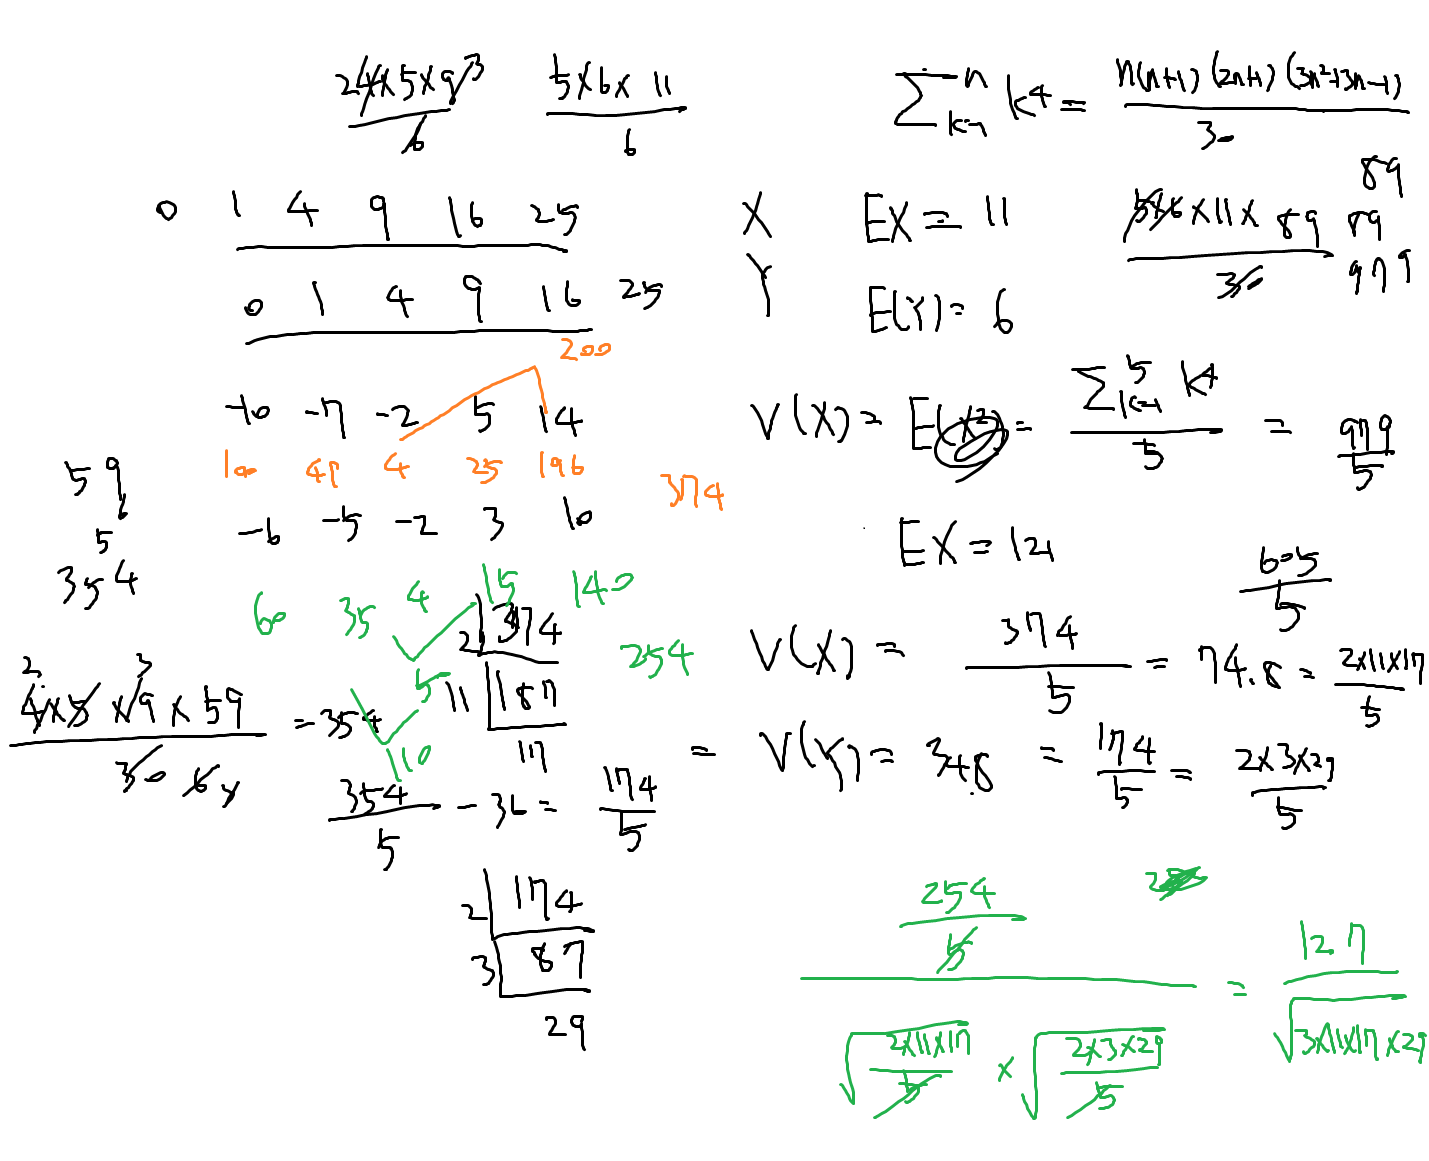
\includegraphics[width=.6\textwidth]{autocorrelation-1}
\end{center}

다음과 같은 생각이 들었다.

\begin{mdframed}
(질문) 어떤 시계열 데이터가 autocorrelation=0을 만족할 수 있을까?
\end{mdframed}

위의 두 예에서는 $X$와 $X'$가 아주 강한 상관관계를 가지고 있었다.
상관계수 값이 작아지려면 어떤 시계열이어야 할까?
자기상관계수(autocorrelation)가 정확히 0이 되는 시계열이 존재할까?
그러니까, 어떤 timestep에 대해서도, 그리고 어떤 lag에 대해서도 상관관계가 0이 되도록 하는 시계열이 존재할 수 있을까?
구글에 아무리 검색을 해봐도 (e.g. ``not autocorrelated time series'') 이것에 대한 말이 없다.
stackoverflow에 물어봐야 할지도 모르겠다.

아래 그림과 같이 여러가지로 시도해봤는데, autocorrelation이 0이 되는 시계열을 발견했다.

\begin{center}
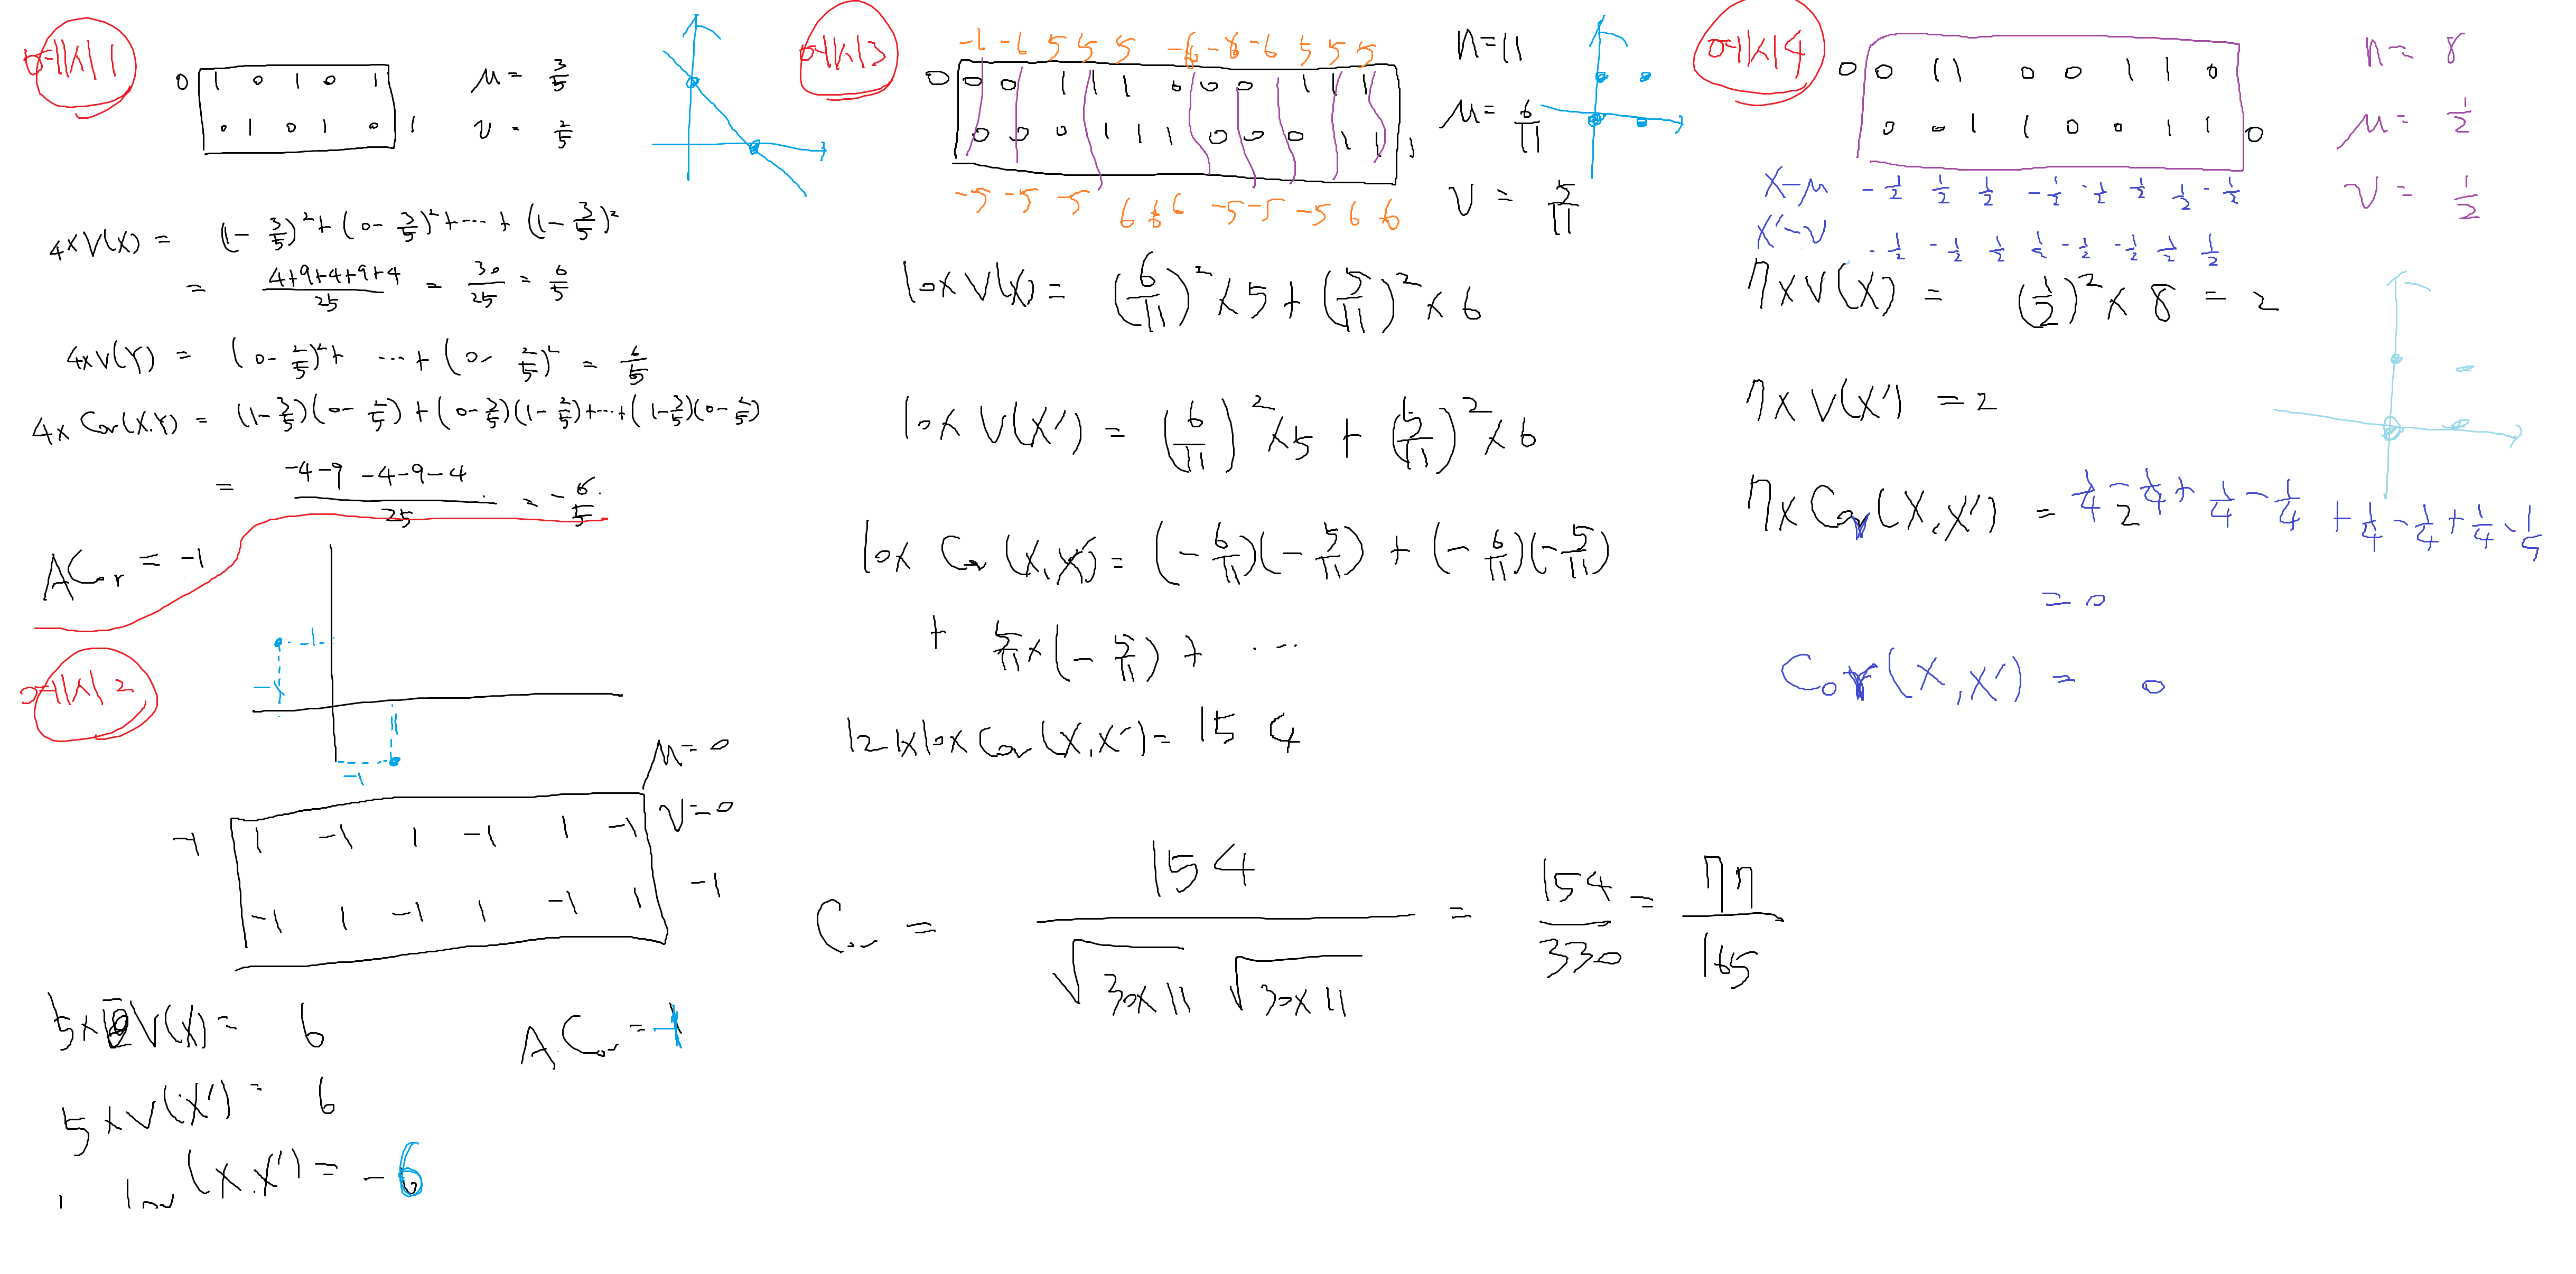
\includegraphics[width=\textwidth]{autocorrelation-2}
\end{center}

맨 오른쪽 계산(예시 4)이다.
이걸 다시 정리해보면 (\(n=8\), \(\mu=\nu=\frac12\))
\begin{center}
\begin{tabular}{c|cccccccccc}
$X $&0&0&1&1&0&0&1&1&0&\\\hline
$X'$& &0&0&1&1&0&0&1&1&0\\\hline
$X-\mu$&$\cdot$&$-\frac12$&$\frac12$&$\frac12$&$-\frac12$&$-\frac12$&$\frac12$&$\frac12$&$-\frac12$&$\cdot$\\\hline
$X'-\nu$&$\cdot$&$-\frac12$&$-\frac12$&$\frac12$&$\frac12$&$-\frac12$&$-\frac12$&$\frac12$&$\frac12$&$\cdot$
\end{tabular}
\end{center}
이다.
표준편차에 해당하는 값을 계산하면
\begin{align*}
\sqrt{\sum_{t=1}^8(x_t-\mu)^2}
&=\sqrt{\frac14\times8}=\sqrt 2\\
\sqrt{\sum_{t=1}^8(x_{t-1}-\nu)^2}
&=\sqrt{\frac14\times8}=\sqrt 2
\end{align*}
이다. 공분산에 해당하는 값을 계산하면
\[\sum_{t=1}^8(x_t-\mu)(x_{t-1}-\nu)=\frac14-\frac14+\frac14-\frac14+\frac14-\frac14+\frac14-\frac14=0.\]
따라서,
\[\text{Cor}(X,X')=\frac{0}{\sqrt2\sqrt2}=0\]
와 같이 계산되고 autocorelation은 0이다.

이것은 조금 더 쉽게 해석될 수도 있다.
위 그림의 예시 1은, 좌표평면 상에 두 점 \((1,0)\), \((0,1)\)을 찍어 그 두 점에 대한 correlation을 계산하는 것이다.
\footnote{조금 더 정확하게는, 점 \((1,0)\) 세 개와 점 \((0,1)\) 두 개, 총 다섯 개의 점에 대한 correlation을 계산한다.}
그러면 당연히, 두 점을 잇는 직선이 존재하고 그 기울기가 음수니까, correlation은 \(-1\)이 될 수밖에 없었다.
마찬가지로, 예시 2는, 두 점 \((1,-1)\), \((-1,1)\)을 찍어 그 두 점에 대한 correlation을 계산하는 것이고, 이번에도 correlation은 \(-1\)이다.
예시 3에서는 네 점 \((0,0)\), \((1,0)\), \((1,1)\), \((0,1)\)의 네 점에 대하여 correalation을 계산하는 것이라고 해석할 수 있는데,
조금 더 정확하게는 4개의 점이라기 보다는, 11개의 점이고, \((0,0)\)은 4개, \((1,0)\)은 2개, \((0,1)\)는 1개, \((1,1)\)는 4개를 고려하는 것이다.
다시 말해, 네 개의 점이기는 하지만 가중치가 부여된 네 개의 점이기 때문에, 이 네 개의 점에 대해서는 correlation이 0인 것이 아니다.
\((0,0)\)과 \((1,1)\)에 가중치가 상대적으로 많이 들어간 셈이므로 correlation은 양수가 되는 것이 맞고, 실제로도 계산이 그렇게 나온다.
마지막으로, 예시 4는 네 점 \((0,0)\), \((1,0)\), \((1,1)\), \((0,1)\)이 equally weighted된 것이라고 볼 수 있다.
이렇게 찍힌 네 점에 대하여는 상관계수가 0이 되는 것이 당연하다.
그래서, 실제 계산도 0이 되었다.

그러면, 실제 강의에서 negative autocorrelation에 대한 내용이 얼추 설명이 된 것 같기도 하다.
그 부분의 캡쳐를 떠오면
\begin{center}
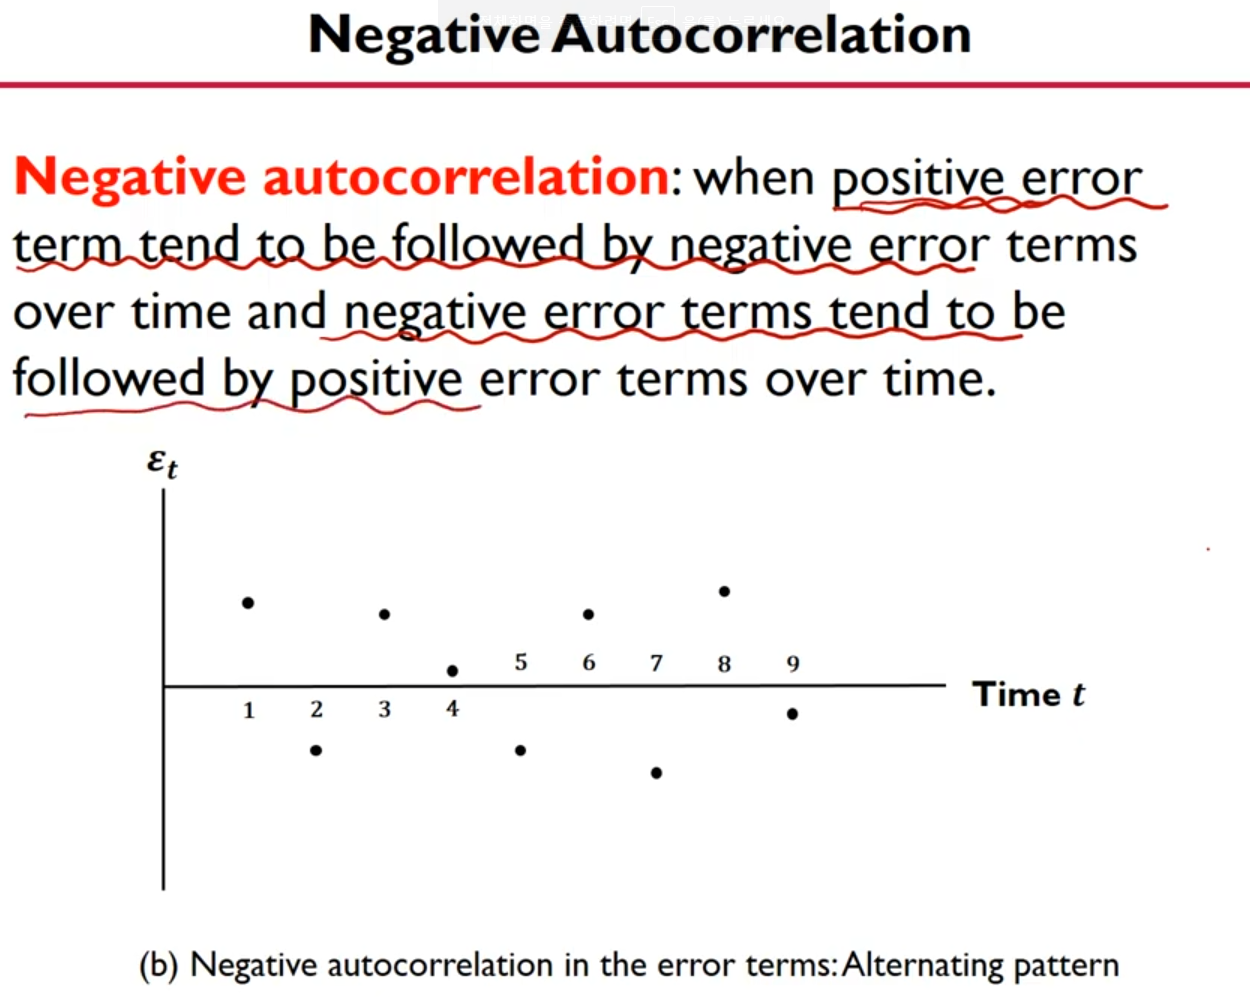
\includegraphics[width=.5\textwidth]{negative_autocorrelation}
\end{center}
인데, 이런 패턴(alternating pattern)의 시계열을 예시 1과 예시 2에서 봤었고, autocorrelation이 $-1$이 된다는 걸 확인했었다.
예시 1과 2에서처럼 일정한 진폭으로 진동하는 게 아니라, 진폭이 조금 변하면서 진동하는 예를 임의로 만들어보면
\begin{center}
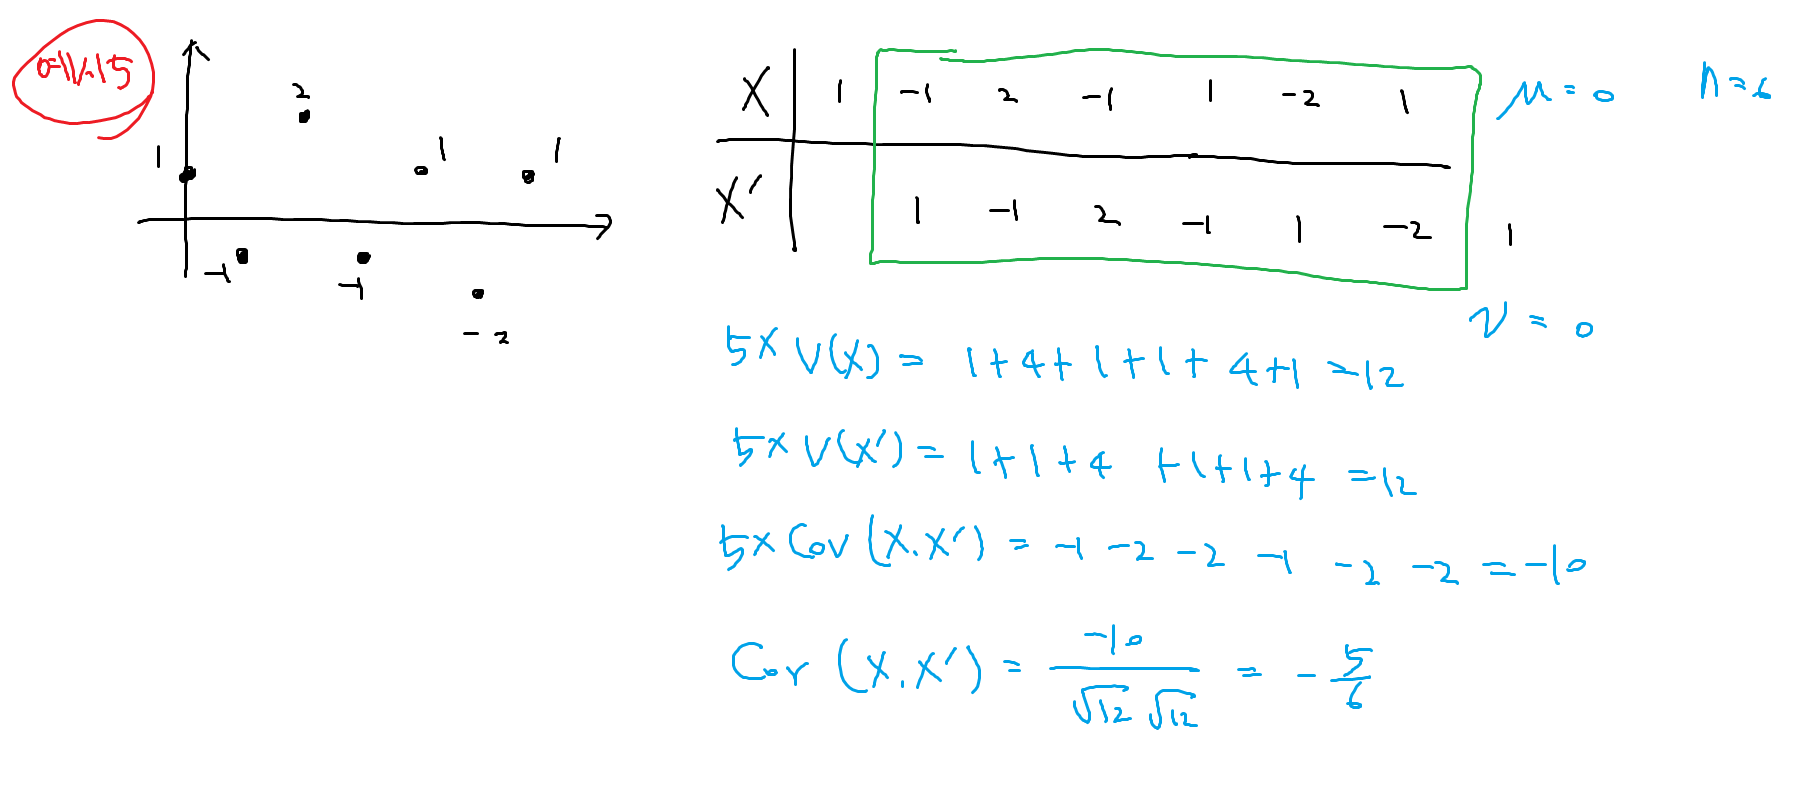
\includegraphics[width=.6\textwidth]{autocorrelation-3}
\end{center}
처럼 만들 수도 있다.

강의에서 positive autocorrelation에 대해 설명한 내용에 관해서는 (아래 캡쳐)
\begin{center}
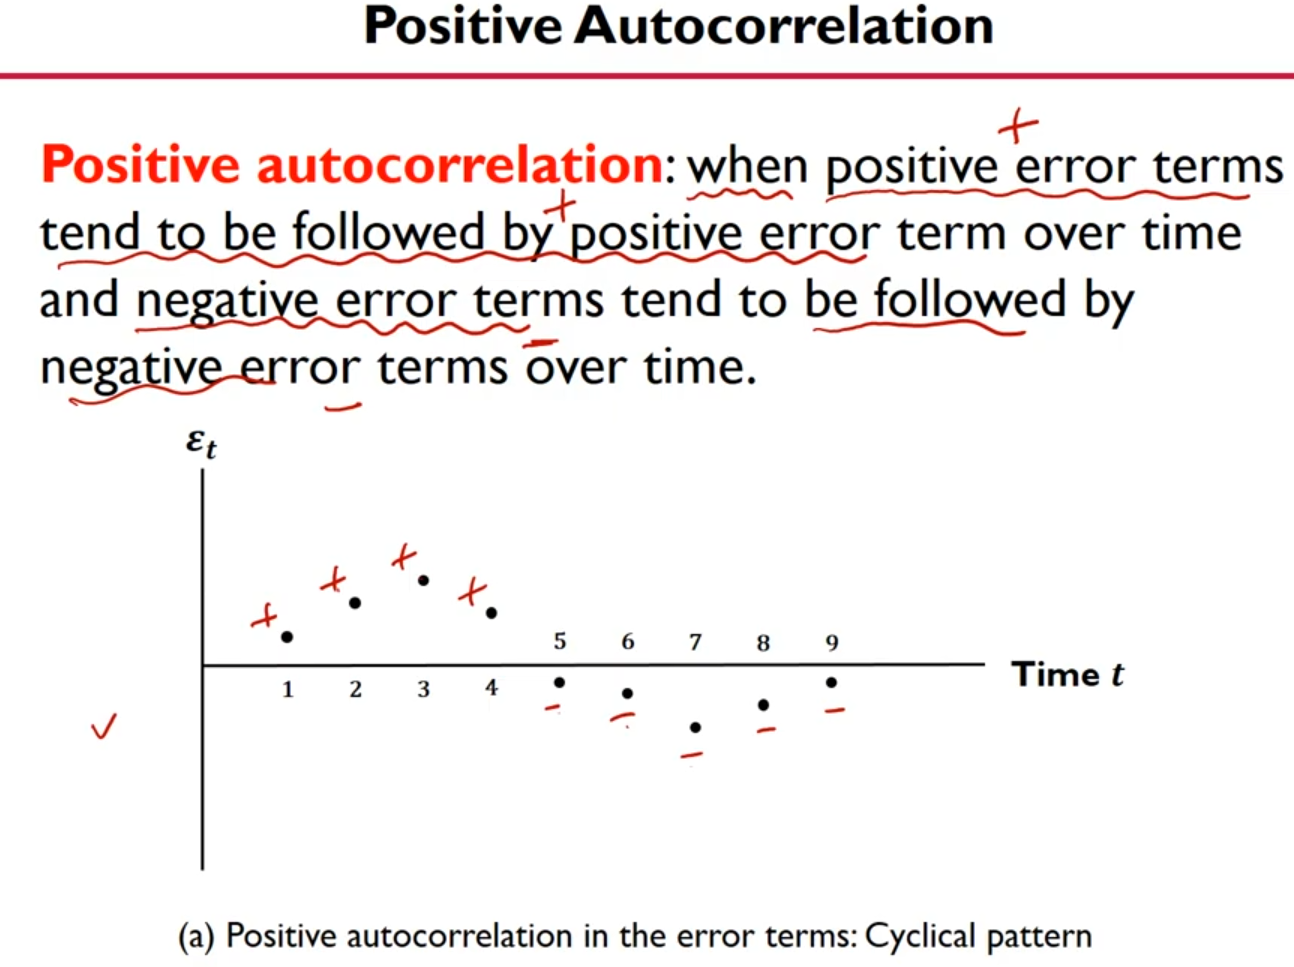
\includegraphics[width=.5\textwidth]{positive_autocorrelation}
\end{center}
예시를 적절하게 든 적이 없다.
마치 사인곡선 같은 예를 들고 있는데 사인곡선 같은건 계산하기가 좀 귀찮을 것 같..으니 간단한 예를 먼저 들면 (예시6)
\begin{center}
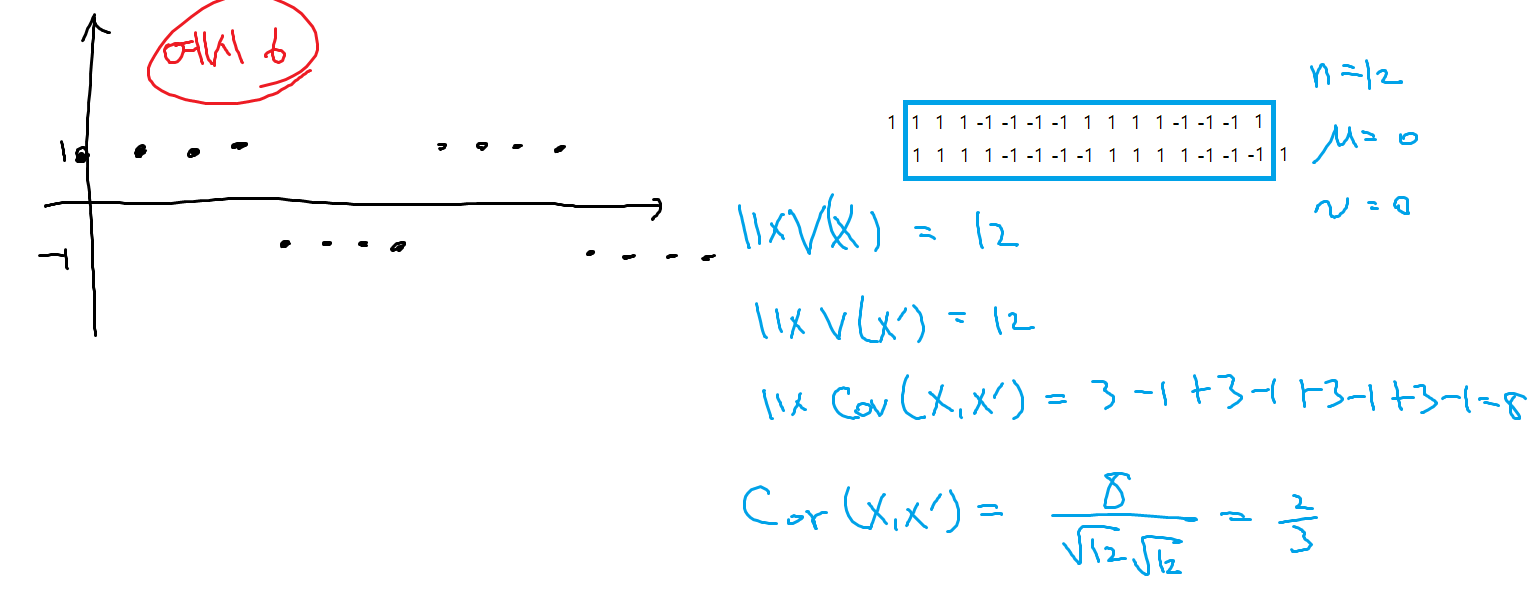
\includegraphics[width=.6\textwidth]{autocorrelation-4}
\end{center}
와 같이 된다.
이건 예시 1, 예시 4, 예시 3을 조금 연장한 것이다.
lag를 1로 고정한 상태에서, 예시 1에서는 alternating 주기가 2였고, 예시 4에서는 alternating 주기가 4였으며, 예시 3에서는 alternating 주기가 6이었다면 이번 예시 6에서는 alternating 주기가 8로 늘어났다.
각각의 자기상관성은 예시 1에서 \(-1\), 예시 4에서 0, 예시 3에서 \(\frac{77}{165}\)쯤 되는 것 같더니 예시 6에서는 \(\frac23\)으로 증가했다.
아마 alternating 주기를 더 늘려가면 자기상관성은 더 커질 것이다.
이것은 강의에서 설명하고 있는, ``양수 이후에 양수가 나오고, 음수 이후에 음수가 나오는'' 경향을 말하는 것 같다.

이번에는 강의 그림에서처럼 사인곡선과 조금 비슷하게 만들어보았다.
\begin{center}
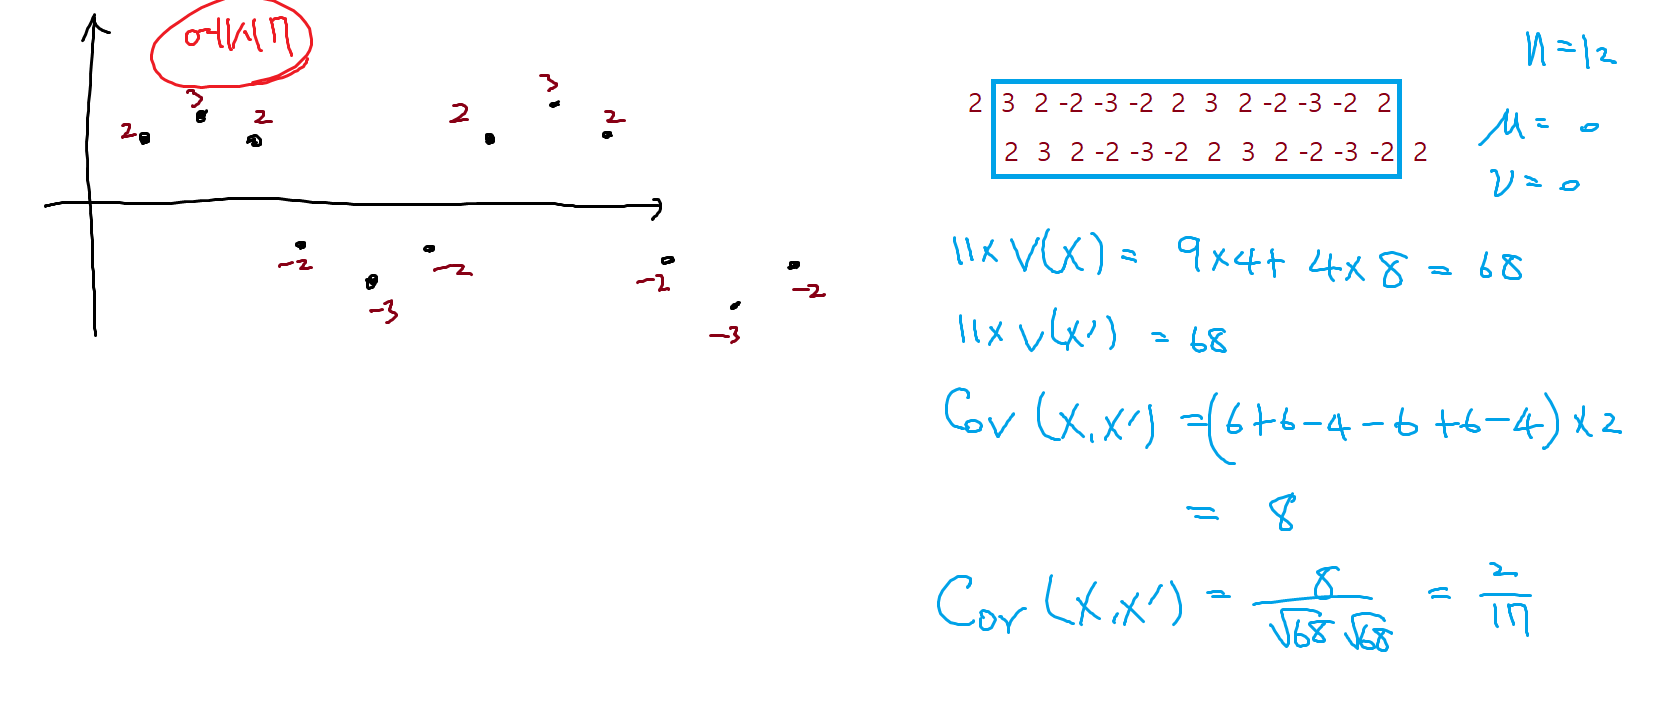
\includegraphics[width=.6\textwidth]{autocorrelation-5}
\end{center}
이 때에도 positive autocorrelation이 계산된다.

%%
\section{Durbin-Watson Test}

어떤 시계열 \(X\)에 대한 오차가 독립 조건을 만족시키는지의 여부를 평가하는 지표로서 Durbin-Watson test가 소개된다.
식 \eqref{DWtest}을 가지고 하는 것인데, 강의에서는 식 \eqref{DWtest}에 대한 조금 정성적인 설명들에만 치중하고 있다.
이 테스트가 어떤 의미를 가지는 지 궁금해서 위키피디아도 찾아봤지만, 만족스러운 설명이 없었던 것 같고, (시계열 분석에 관한 가장 유명한 책인 것 같은) Shumway의 \emph{Time Series Analysis and Its Applications With \texttt R Examples}라는 책을 읽어보고는 있지만, 아무래도 이 테스트가 설명되어 있지는 않은 것 같다.
(하지만 더 읽어봐야 한다.)
아무튼 그래서, 내 나름대로 \eqref{DWtest}의 의미를 파악해보려고 해보았다.

%%%
\subsection{autocorrelation applied to the residual term}
지금까지, 어떤 시계열 데이터에 대한 자기상관성(autocorrelation)에 대해 말했다.
하지만, 5번 각주에서 말했듯이, 우리가 관심있는 것은 error term(오차, \(e_t\))의 자기상관성이고, 실제로는 error term을 알 수 없으니 대신에 residual term(잔차, \(\epsilon_t\))의 자기상관성을 다룬다.
residual term들의 수열을 그냥 \(\epsilon\)이라고 하자.
\[\epsilon=\{\epsilon_t:t=1,2,\cdots,n\}\]
그리고 \(\epsilon\)을 한 timestep 민 것을 \(\epsilon'\)이라고 하자 (first order; lag=1)
\[\epsilon'=\{\epsilon_{t+1}:t=1,2,\cdots,n\}.\]
그러면, 여기에서 구해야 하는, residual term의 autocorrelation \(\rho_1(\epsilon)\)은  다음과 같이 표현된다.
\begin{equation}\label{autocorrelation_of_residual}
\begin{aligned}
\rho_1(\epsilon)
&=\text{Cor}(\epsilon,\epsilon')\\
&=\frac{\sum_{t=2}^n(\epsilon_t-\mu)(\epsilon_{t-1}-\nu)}{\sqrt{\sum_{t=2}^n(\epsilon_t-\mu)^2}\sqrt{\sum_{t=2}^n(\epsilon_{t-1}-\nu)^2}}
\end{aligned}
\end{equation}

%%%
\subsection{Durbin-Watson Test}
그런데 Durbin-Watson Test에서는 위의 값과는 다른 값을 고려한다.
아래의 값이다.
\begin{equation}\label{DWtest}
d = \frac{\sum_{i=2}^n(\epsilon_i-\epsilon_{i-1})^2}{\sum_{i=1}^n{\epsilon_i}^2}
\end{equation}
%residual의 독립성이 보장되는가 하는 것을 말하고자 하므로 식 \eqref{autocorrelation_of_residual}을 사용하는 게 맞을 것 같다.
이것을 식 \eqref{autocorrelation_of_residual}과 비교해보자.
\eqref{autocorrelation_of_residual}에서 잔차의 평균은 0으로 가정하기로 했으니 \(\mu=\nu=0\)으로 놓을 수 있을 것이다.
또한, \(\epsilon_t\)의 분산은 \(t\)에 따라서 달라지지 않는다고도 했으니, 분모의 두 항은 같다고도 할 수 있을 것이다.
그러니 \eqref{autocorrelation_of_residual}을
\begin{equation}\label{autocorrelation_of_residual_modified}
\rho_1(\epsilon)=\frac{\sum_{t=2}^n\epsilon_t\epsilon_{t+1}}{\sum_{t=2}^n{\epsilon_t}^2}
\end{equation}
로 바꿀 수 있다.
그러면 식이 \eqref{DWtest}와 조금 비슷해지기는 했다.
index가 $i$로 써져있는 것은 크게 문제가 되지 않고, 분모에서 $i$의 범위가 1에서 \(n\)까지인 것도 \eqref{autocorrelation_of_residual_modified}에서 $t$의 범위가 1에서 \(n-1\)까지인 것과 (조금 다르지만) 거의 비슷하다.
다만, 분자가 \((\epsilon_i-\epsilon_{i-1})^2\) 꼴인 것은 \(\epsilon_t\epsilon_{t+1}\)인 것과 많이 다르다.
식 \eqref{DWtest}를 \eqref{autocorrelation_of_residual_modified}의 형태로 바꾸어서, \(d\)와 \(\rho_1(\epsilon)\) 사이의 관계를 살펴보면,
\begin{equation}\label{relation_between_d_and_rho}
\begin{aligned}
d
&=\frac{\sum_{t=2}^n(\epsilon_{t+1}-\epsilon_t)^2}{\sum_{t=2}^n{\epsilon_t}^2}\\
&=\frac{\sum_{t=2}^n{\epsilon_{t+1}}^2-2\sum_{t=2}^n\epsilon_{t+1}\epsilon_t+\sum_{t=2}^n{\epsilon_t}^2}{\sum_{t=2}^n{\epsilon_t}^2}\\
&=2-2\frac{\sum_{t=2}^n\epsilon_{t+1}\epsilon_t}{\sum_{t=2}^n{\epsilon_t}^2}\\
&\approx 2-2\rho_1(\epsilon)
\end{aligned}
\end{equation}
\(\rho_1(\epsilon)\)이 0에 가깝게 되면 residual term의 autocorrelation이 0에 가깝게 되는 것이고, 잔차들이 서로 독립이라는 것을 의미한다.
그것은 \(d\)의 관점에서 보면, \(d\)의 값이 2에 가까워지는 것에 대응된다.
교과서같은 걸 보지 않아서 이런 계산이 정말로 Durbin-Watson test와 연관이 있는지 확실하게는 모르겠지만, 아래 정황상 맞는 것 같다.

\begin{center}
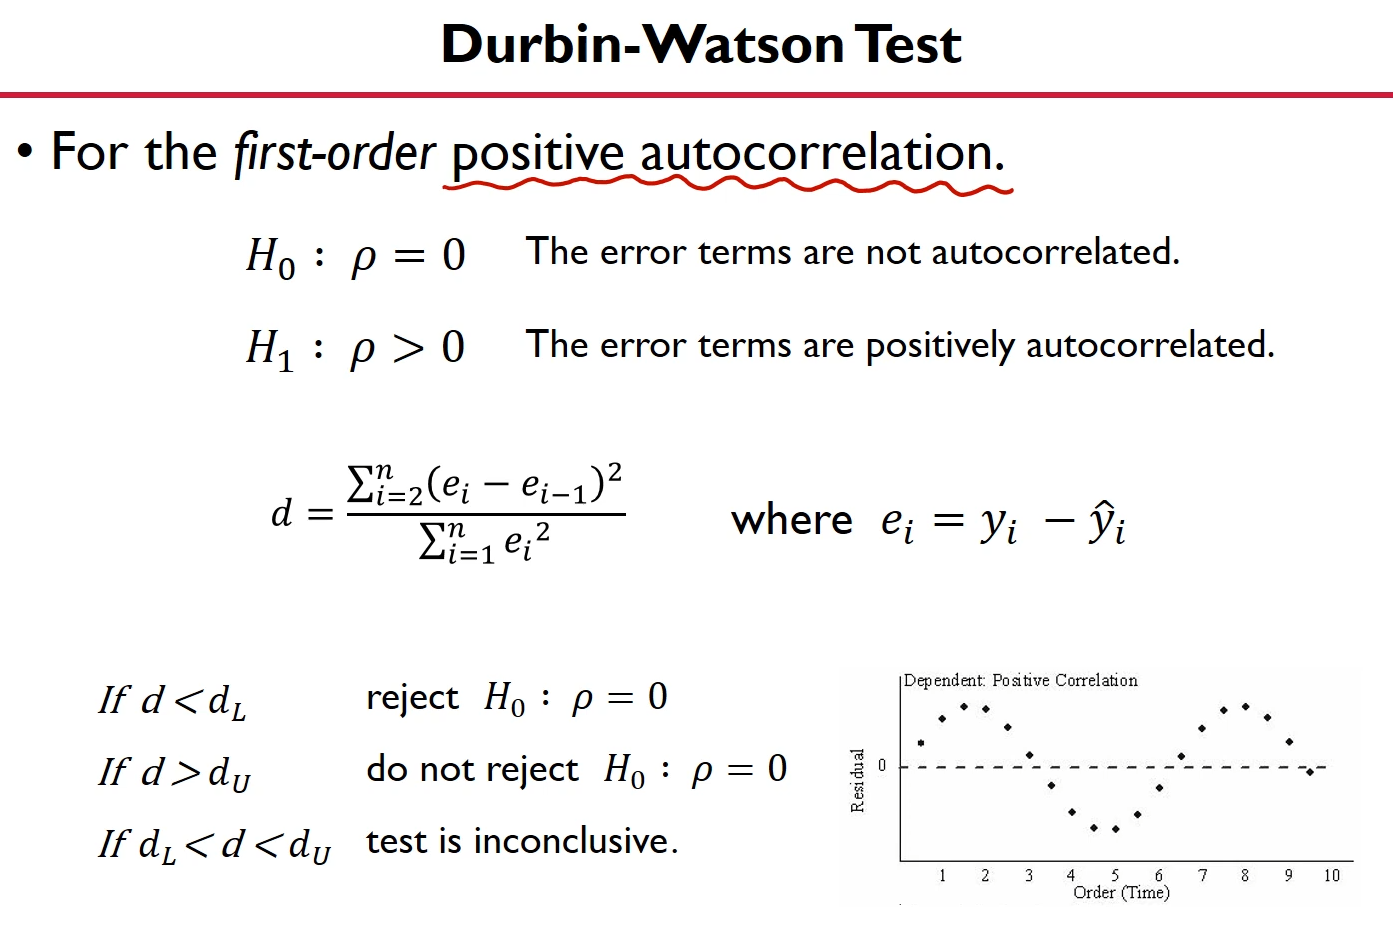
\includegraphics[width=.5\textwidth]{positively_autocorrelated_test}
\end{center}

강의의 32분 40초쯤의 설명에서 \(d\)가 작으면 (대립가설을 택하여) `\(X\)가 positively autocorrelated 하다.'라는 결론을 내린다고 되어 있고, \(d\)가 크면 (귀무가설을 택하여) `\(X\)가 not autocorrelated하다.'라는 결론을 내린다고 되어 있다.
실제로, 식 \eqref{relation_between_d_and_rho}에서 \(d\)가 2보다 작다는 것은 \(\rho_1(\epsilon)\)이 양수라는 것이고, 정말로 positively autocorrelated라는 것을 뜻한다.
영상에서는 \(d_L\)과 \(d_U\)를 설정해서 `positively autocorrelated test'를 소개하고 있는 것 같다.
아래첨자로 사용된 \(L\)과 \(U\)는 각각 lower, upper를 말하는 것 같다.
이 \(d_L\)과 \(d_U\)들은 임계값(threshold)의 역할을 한다.

만약, \(d_L\)을 2보다 조금 작은 값으로 잡는다면, \(d\)가 \(d_L\)보다 작다는 것이, \(\rho_1(\epsilon)\)이 특정한 양수보다 크다는 것을 의미하고, 이것은 \(X\)가 어느 정도 positively autocorrelated 되어 있다는 것을 말한다고 볼 수 있다.
그리고 \(d_U\)를 \(d_L\)보다는 조금 크면서 \(2\)보다는 작은 값으로 적당히 잡는다면, \(d\)가 \(d_L\)보다 크다는 것이, \(\rho_1(\epsilon)\)이 특정한 양수\footnote{앞 문장에서의 `특정한 양수'보다는 조금 작은 양수} 보다 작다는 것을 의미하고, 이것은 \(X\)가 꼭 positively autocorrelated 되어있다고는 볼 수 없다는 걸 이야기한다고 말할 수 있다.
그렇다고 해서 negatively autocorrelated라는 것은 아니다.
negatively autocorrelated 되어 있는지의 여부는 `negatively autocorrelated test'를 통해서 따로 해야 할 것이다.

\begin{center}
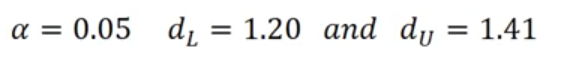
\includegraphics[width=.3\textwidth]{d_L_and_d_U}
\end{center}

다음 슬라이드 (34분 30초경)의 표에서는 적당한 \(d_L\)과 \(d_U\)의 값들의 목록을 표시하고 있다.
앞 문단에서 \(d_L\)은 2보다 조금 작은 값, \(d_U\)는 \(d_L\)보다는 크면서 2보다는 작은 값이라고 했엇는데, 그 다음 슬라이드에서 특정한 경우에 대해서는 \(d_L=1.20\), \(d_U=1.41\)로 두고 있다.
그러니까 위의 설명은 맞는 것 같다.

\begin{center}
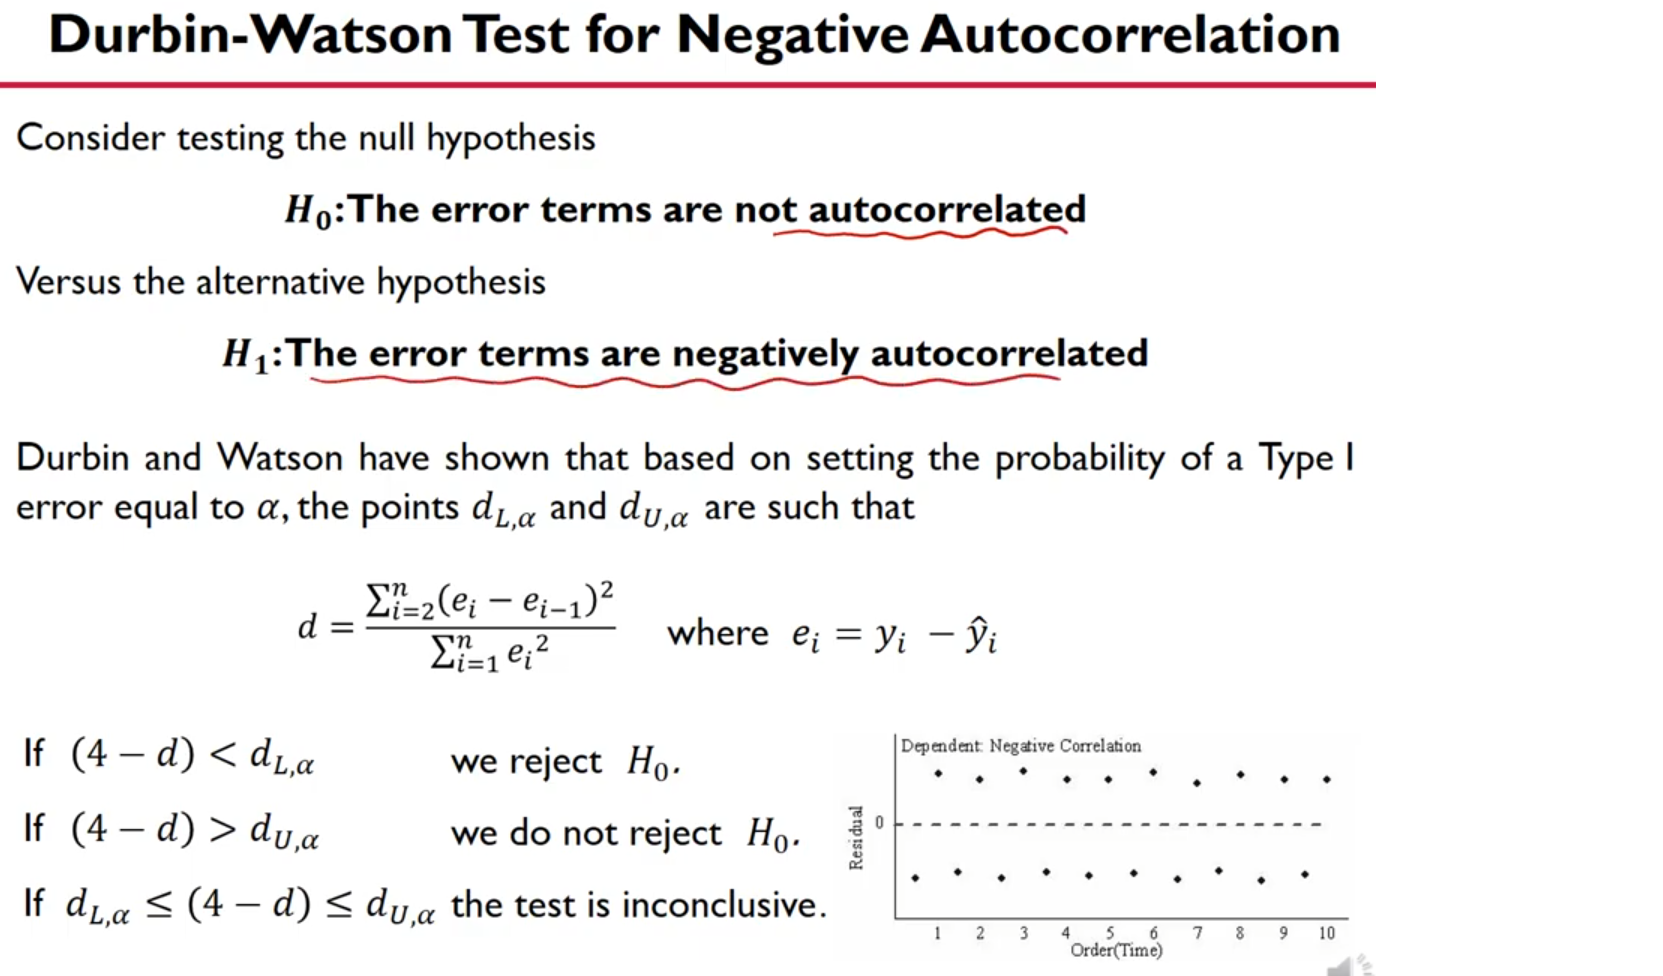
\includegraphics[width=.5\textwidth]{negatively_autocorrelated_test}
\end{center}

negatively autocorrelated test에 대한 설명은 위의 그림과 같다.
여기에서는 \(d\)가 아닌 \(4-d\)를 사용하는데 \eqref{relation_between_d_and_rho}을 변형하면
\[4-d=2+2\rho_1(\epsilon)\]
이 된다.
이번에는 \(d_L\)과 \(d_U\)의 값이 예를 통해 제시되고 있지는 않다.
하지만 아까와 같은 \(d_L=1.20\), \(d_U=1.41\)로 생각하고 해석해보면 다음과 같다.
만약 \(4-d\)가 \(d_L=1.20\)보다 작으면, 그것은 \(2+2\rho_1(\epsilon)<1.20\), \(\rho_1(\epsilon)<-0.4\)을 의미한다.
그러니까, \(\rho_1(\epsilon)\)이 음수이면서, 그냥 음수도 아니고 일정한 절댓값(0.4)보다 크게 음수로 나타나고 있다.
이럴 때에, \(X\)가 negatively autocorrelated하다고 판단한다.
또한, 만약 \(4-d\)가 \(d_U=1.41\)보다 크면, 그것은 \(2+2\rho_1(\epsilon)>1.41\), \(\rho_1(\epsilon)>-0.295\)를 의미힌다.
그러니까, \(\rho_1(\epsilon)\)이 음수일 수도 있기는 하지만, 아주 절댓값이 큰 음수는 아니라는 것을, 그러니까 \(X\)가 negatively autocorrelated라고 판단할 만큼은 아니라는 것을 알 수 있다.

마지막으로, Durbin-Watson test에 대한 comment를 그냥 캡쳐해서 첨부해보았다.

\begin{center}
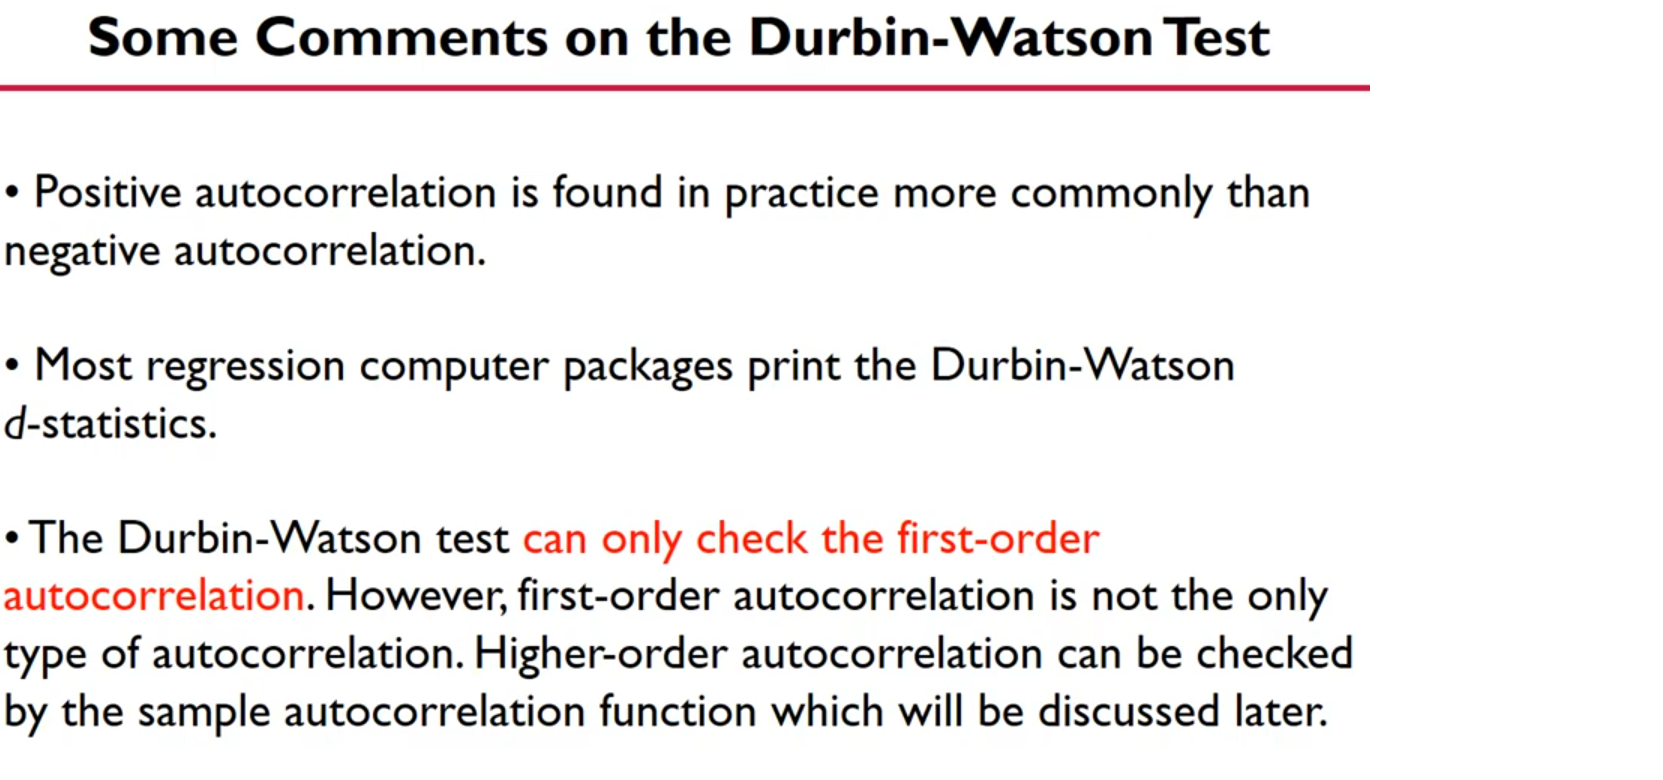
\includegraphics[width=.5\textwidth]{comment_on_DWtest}
\end{center}

%%
\section{Increasing Seasonal Variations}
마지막 주제로서, seasonal variation이 점차적으로 증가하는 다음 그림과 같은 상황을 이야기하고 있다.
\begin{center}
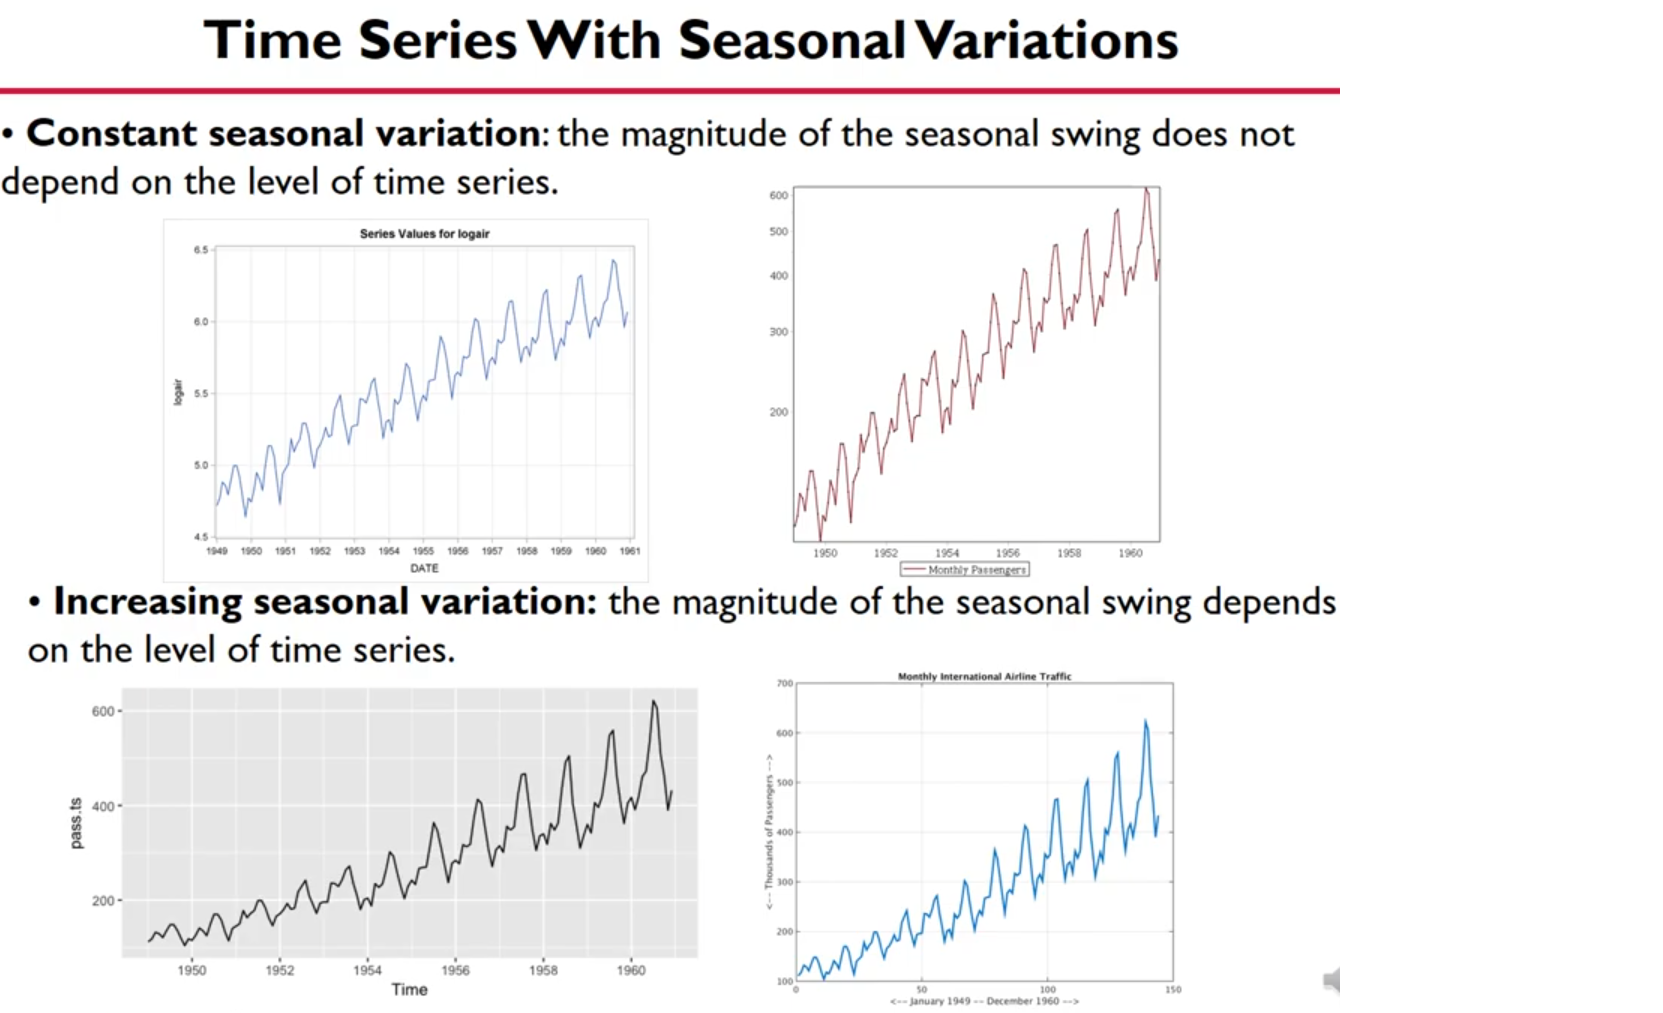
\includegraphics[width=.5\textwidth]{increasing_seasonal_variation}
\end{center}
increasing seasonal variation인 경우는 데이터를 다루기가 어렵다고 한다.
이것을 constant seasonal variation으로 바꾸기 위해서 두 가지 방법을 쓰고 있다.

increasing seasonal variation의 두 time series는 그 trend가 이차함수처럼 혹은 지수함수처럼 증가하는 것을 관찰할 수 있다.
그러니까, 두 timeseries에 \(y=\sqrt x\)나 \(y=\log x\) 같은 것을 취해주면, trend를 선형적인(직선의) 모습으로 바꿀수 있을 것이다.
trend가 선형적인 모습을 띄게 되면 seasonal swing 또한 자연스럽게 일정한 값을 가지게 될 것이다.
그래서 아래의 두 가지 방법을 쓰는 게 아닌가 한다.
\begin{center}
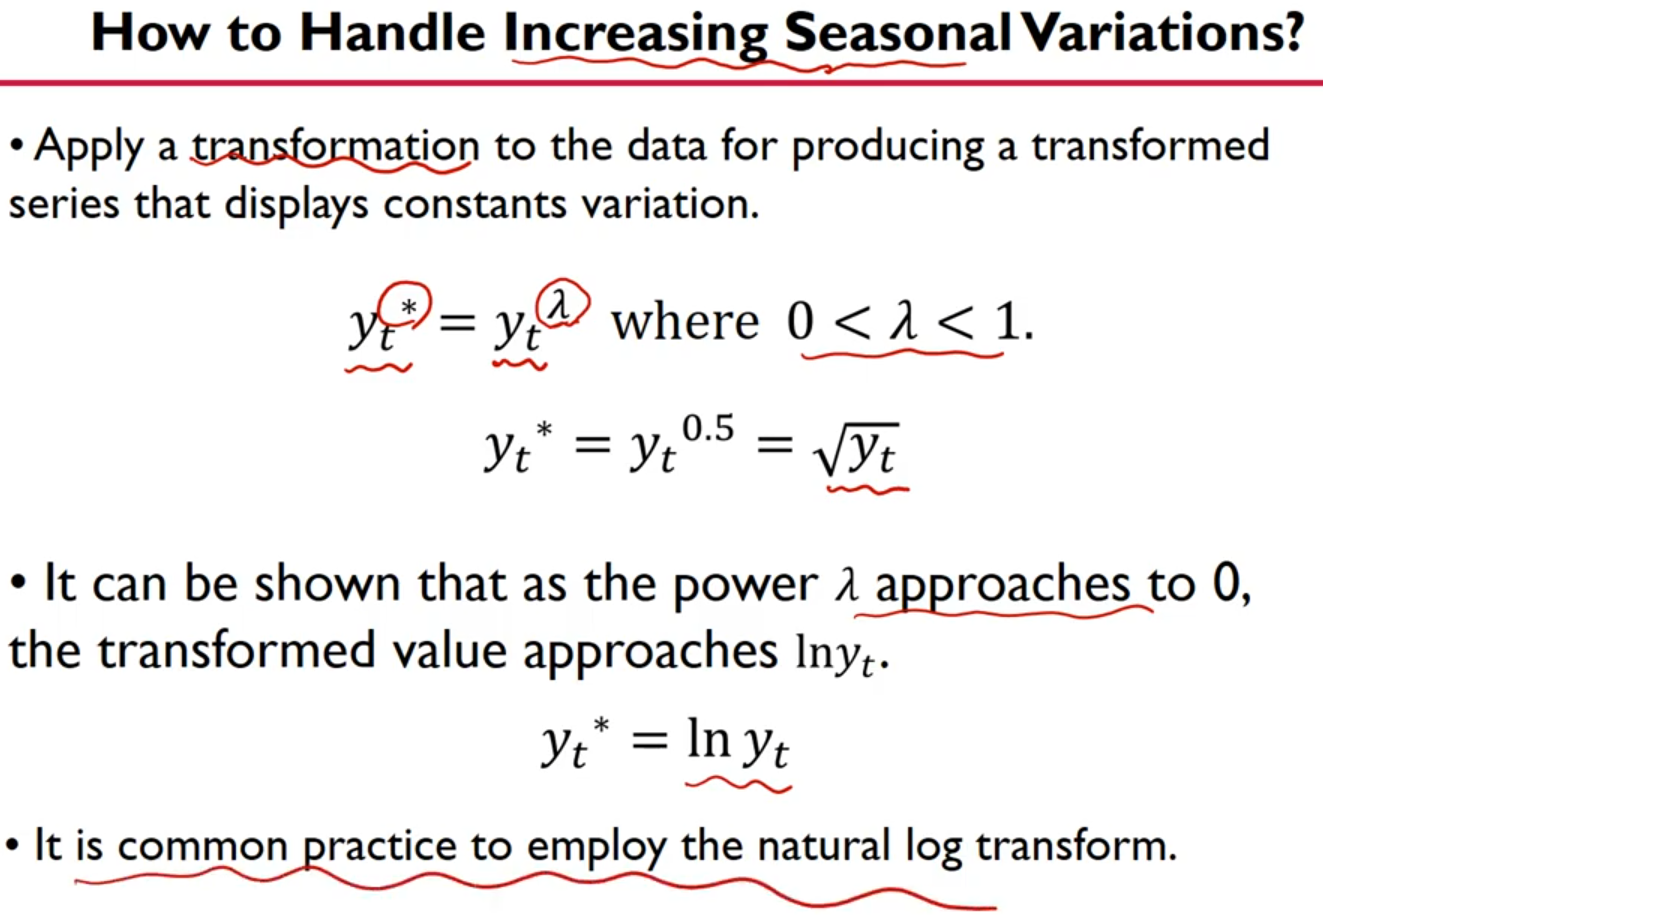
\includegraphics[width=.5\textwidth]{two_transforms}
%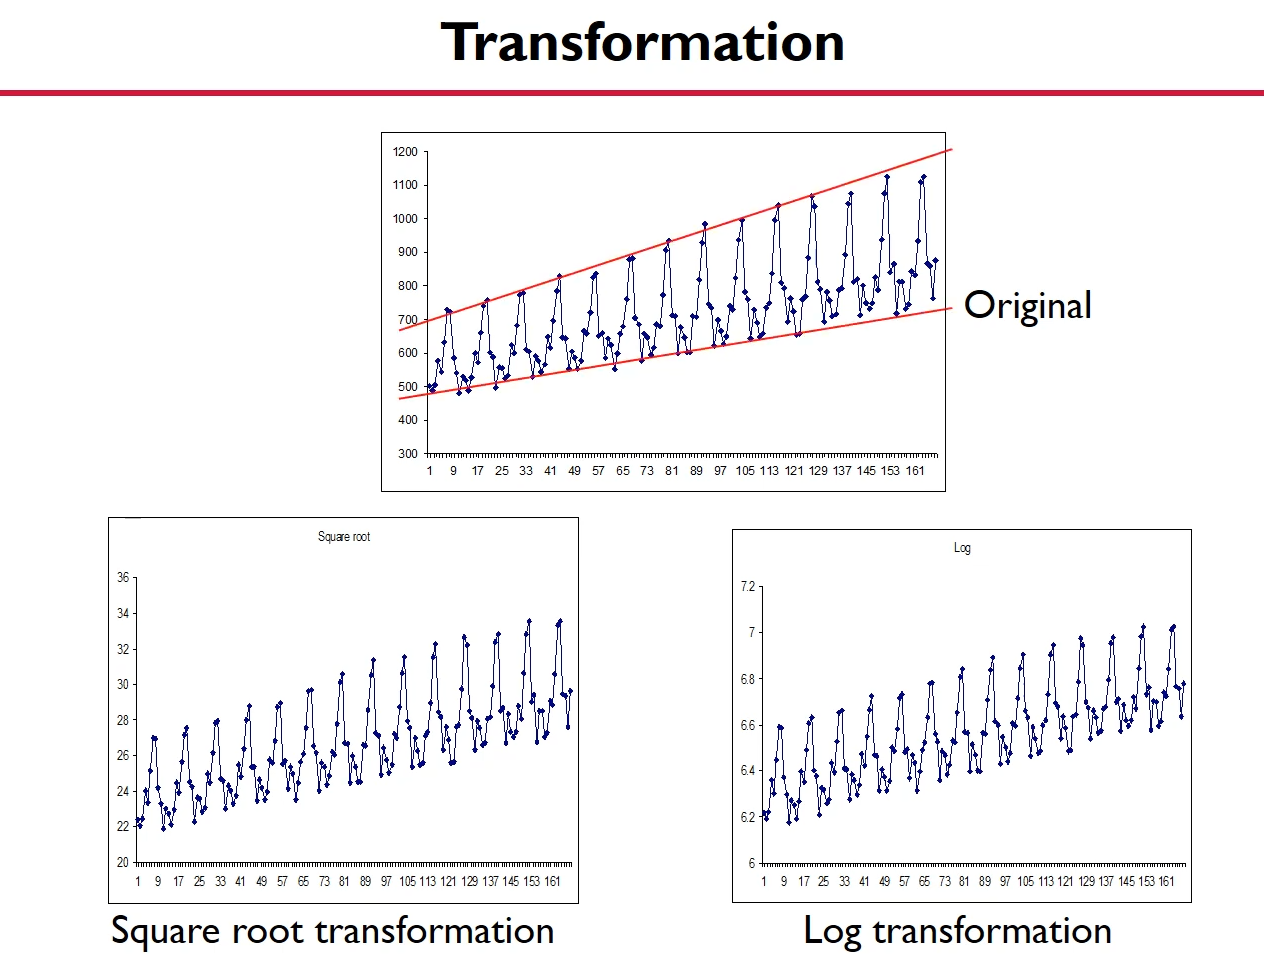
\includegraphics[width=.5\textwidth]{after_transforms}
\end{center}



\end{document}